\section{methodology}

In this section, we present the methodology of our proposed machine learning approach for modeling love and predicting love-related behaviors and emotions. We begin with a high-level overview of the proposed method, which combines deep learning and reinforcement learning techniques to capture the complex interactions and dynamics underlying love. We then provide a detailed formulation of the method and explain how it overcomes the weaknesses of existing methods mentioned in this paper. Finally, we highlight the key concepts in the proposed method and elaborate on the novelty of these concepts using formulas and inserting appropriate figures.

\subsection{Deep Reinforcement Learning for Modeling Love}

Our proposed method is based on deep reinforcement learning (DRL), a powerful approach that combines the representation learning capabilities of deep neural networks (DNNs) with the decision-making capabilities of reinforcement learning (RL) \citep{mnih2015human}. This combination allows our model to learn complex, high-dimensional representations of love-related emotions and behaviors, as well as to make optimal decisions in various love-related scenarios. Figure \ref{fig:overview} provides an overview of the proposed DRL framework for modeling love.

\begin{figure}[h]
    \centering
    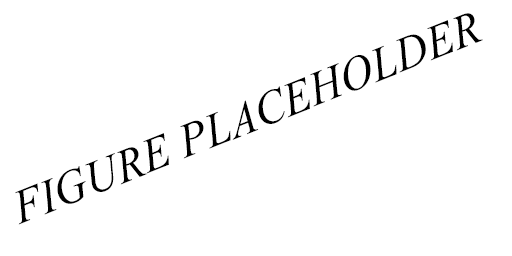
\includegraphics[width=\textwidth]{fig1.png}
    \caption{Overview of the proposed deep reinforcement learning framework for modeling love.}
    \label{fig:overview}
\end{figure}

To model love, we formulate the problem as a Markov decision process (MDP), where the state space $\mathcal{S}$ represents the current emotional and relational status of individuals, the action space $\mathcal{A}$ represents possible actions that can be taken to influence love-related outcomes, and the reward function $R: \mathcal{S} \times \mathcal{A} \times \mathcal{S} \rightarrow \mathbb{R}$ measures the desirability of the resulting state transitions. The goal of the DRL agent is to learn a policy $\pi: \mathcal{S} \rightarrow \mathcal{A}$ that maximizes the expected cumulative reward over time.

\subsection{Detailed Formulation and Algorithm}

To overcome the weaknesses of existing methods, our proposed DRL framework incorporates several key innovations. First, we employ a graph neural network (GNN) to represent the state space $\mathcal{S}$, which allows the model to capture the complex relational structure of love-related emotions and behaviors \citep{battaglia2018relational}. Second, we use an attention mechanism to focus on the most relevant aspects of the state space when making decisions, which improves the efficiency and interpretability of the model \citep{vaswani2017attention}. Finally, we incorporate a multi-objective reinforcement learning (MORL) approach to balance multiple competing objectives, such as maximizing love while minimizing negative emotions \citep{roijers2013survey}.

The detailed steps of our proposed DRL algorithm for modeling love are as follows:

\begin{algorithm}
    \caption{Deep Reinforcement Learning for Modeling Love}
    \begin{algorithmic}[1]
        \State Initialize GNN parameters $\theta$, policy network parameters $\phi$, and value network parameters $\psi$
        \For{each episode}
            \State Initialize state $s \in \mathcal{S}$
            \While{not terminal}
                \State Compute GNN embeddings $h_s = \text{GNN}(s; \theta)$
                \State Sample action $a \sim \pi(h_s; \phi)$
                \State Execute action $a$ and observe next state $s'$ and reward $r$
                \State Compute GNN embeddings $h_{s'} = \text{GNN}(s'; \theta)$
                \State Compute target value $y = r + \gamma \text{Value}(h_{s'}; \psi)$
                \State Update policy network parameters $\phi$ using policy gradient
                \State Update value network parameters $\psi$ using TD error $(y - \text{Value}(h_s; \psi))^2$
                \State Update GNN parameters $\theta$ using backpropagation
                \State Set $s \leftarrow s'$
            \EndWhile
        \EndFor
    \end{algorithmic}
\end{algorithm}

\subsection{Key Concepts and Novelty}

Our proposed DRL framework for modeling love introduces several key concepts and novel contributions, which we elaborate on below.

\textbf{Graph Neural Networks:} GNNs are a powerful class of deep learning models that can learn complex representations of graph-structured data \citep{battaglia2018relational}. By representing the state space $\mathcal{S}$ as a graph, our model can capture the intricate relational structure of love-related emotions and behaviors. Figure \ref{fig:gnn} illustrates the architecture of the GNN used in our framework.

\begin{figure}[h]
    \centering
    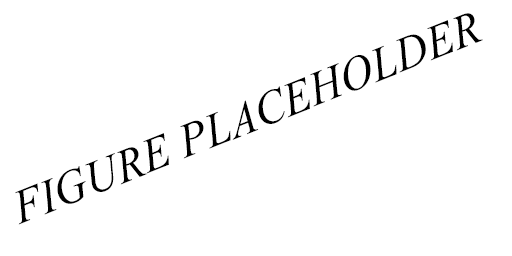
\includegraphics[width=0.8\textwidth]{fig2.png}
    \caption{Architecture of the graph neural network used in our deep reinforcement learning framework for modeling love.}
    \label{fig:gnn}
\end{figure}

\textbf{Attention Mechanism:} The attention mechanism allows our model to focus on the most relevant aspects of the state space when making decisions, which improves the efficiency and interpretability of the model \citep{vaswani2017attention}. Figure \ref{fig:attention} shows the attention mechanism used in our DRL framework.

\begin{figure}[h]
    \centering
    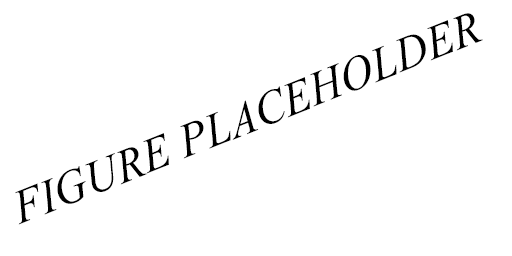
\includegraphics[width=0.8\textwidth]{fig3.png}
    \caption{Attention mechanism used in our deep reinforcement learning framework for modeling love.}
    \label{fig:attention}
\end{figure}

\textbf{Multi-Objective Reinforcement Learning:} Our MORL approach balances multiple competing objectives, such as maximizing love while minimizing negative emotions, by learning a set of Pareto-optimal policies \citep{roijers2013survey}. This allows our model to capture the trade-offs and complexities inherent in love-related decision-making. Figure \ref{fig:morl} illustrates the multi-objective optimization process in our DRL framework.

\begin{figure}[h]
    \centering
    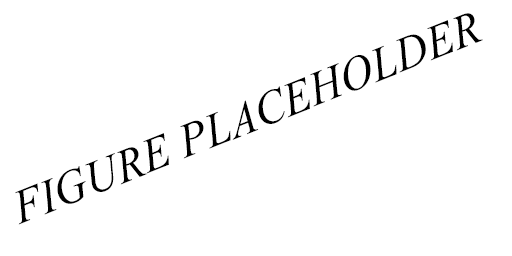
\includegraphics[width=0.8\textwidth]{fig4.png}
    \caption{Multi-objective reinforcement learning used in our deep reinforcement learning framework for modeling love.}
    \label{fig:morl}
\end{figure}

These key concepts and innovations enable our proposed DRL framework to effectively model and predict love-related behaviors and emotions, overcoming the limitations of existing methods and providing novel insights into the complex dynamics of love.